
%%%%%%%%%%%%%%%%%%%%%%%%%%%%%%%%%%%%%%%%%%%%%%%%%%%%%%%%%%%%%%%%%%%%%%%%%%%%%%%%%%%%%%%%%%%%%%%%%
%
% Document:      RiskProcess
%
%%%%%%%%%%%%%%%%%%%%%%%%%%%%%%%%%%%%%%%%%%%%%%%%%%%%%%%%%%%%%%%%%%%%%%%%%%%%%%

\documentclass{article}

\usepackage{times,layouts}
\usepackage{tikz,hyperref,amsmath}
\usetikzlibrary{positioning,arrows,shapes,decorations.shapes,shapes.arrows}
\usetikzlibrary{backgrounds,calc}

\usepackage[paperwidth=18cm,paperheight=185mm,
left=-2mm,top=3mm,bottom=0mm,right=0mm,
noheadfoot,marginparwidth=0pt,includemp=false,
textwidth=30cm,textheight=50mm]{geometry}


\newcommand\showpage{%
\setlayoutscale{0.5}\setlabelfont{\tiny}\printheadingsfalse\printparametersfalse
\currentpage\pagedesign}

\hypersetup{pdftitle={DM risk process }, pdfsubject={Diagram illustrating the
 risk process in  LSST DM Group}, pdfauthor={ William O'Mullane}}



\tikzstyle{rbox}=[rectangle, rounded corners=3pt, draw=black, fill=brown!20
, very thick, minimum height=2cm, inner sep=2pt, text centered, text width=3cm]

\tikzstyle{abox}=[rectangle, minimum height=2cm, color=red, inner sep=2pt, text centered, text width=3cm]

\tikzstyle{pline}=[->, line width=3pt, brown]
\tikzstyle{pdline}=[->, line width=3pt, dashed, brown]
\tikzstyle{rline}=[->, line width=4pt, shorten >=18pt, dashed, red!70]
\begin{document}

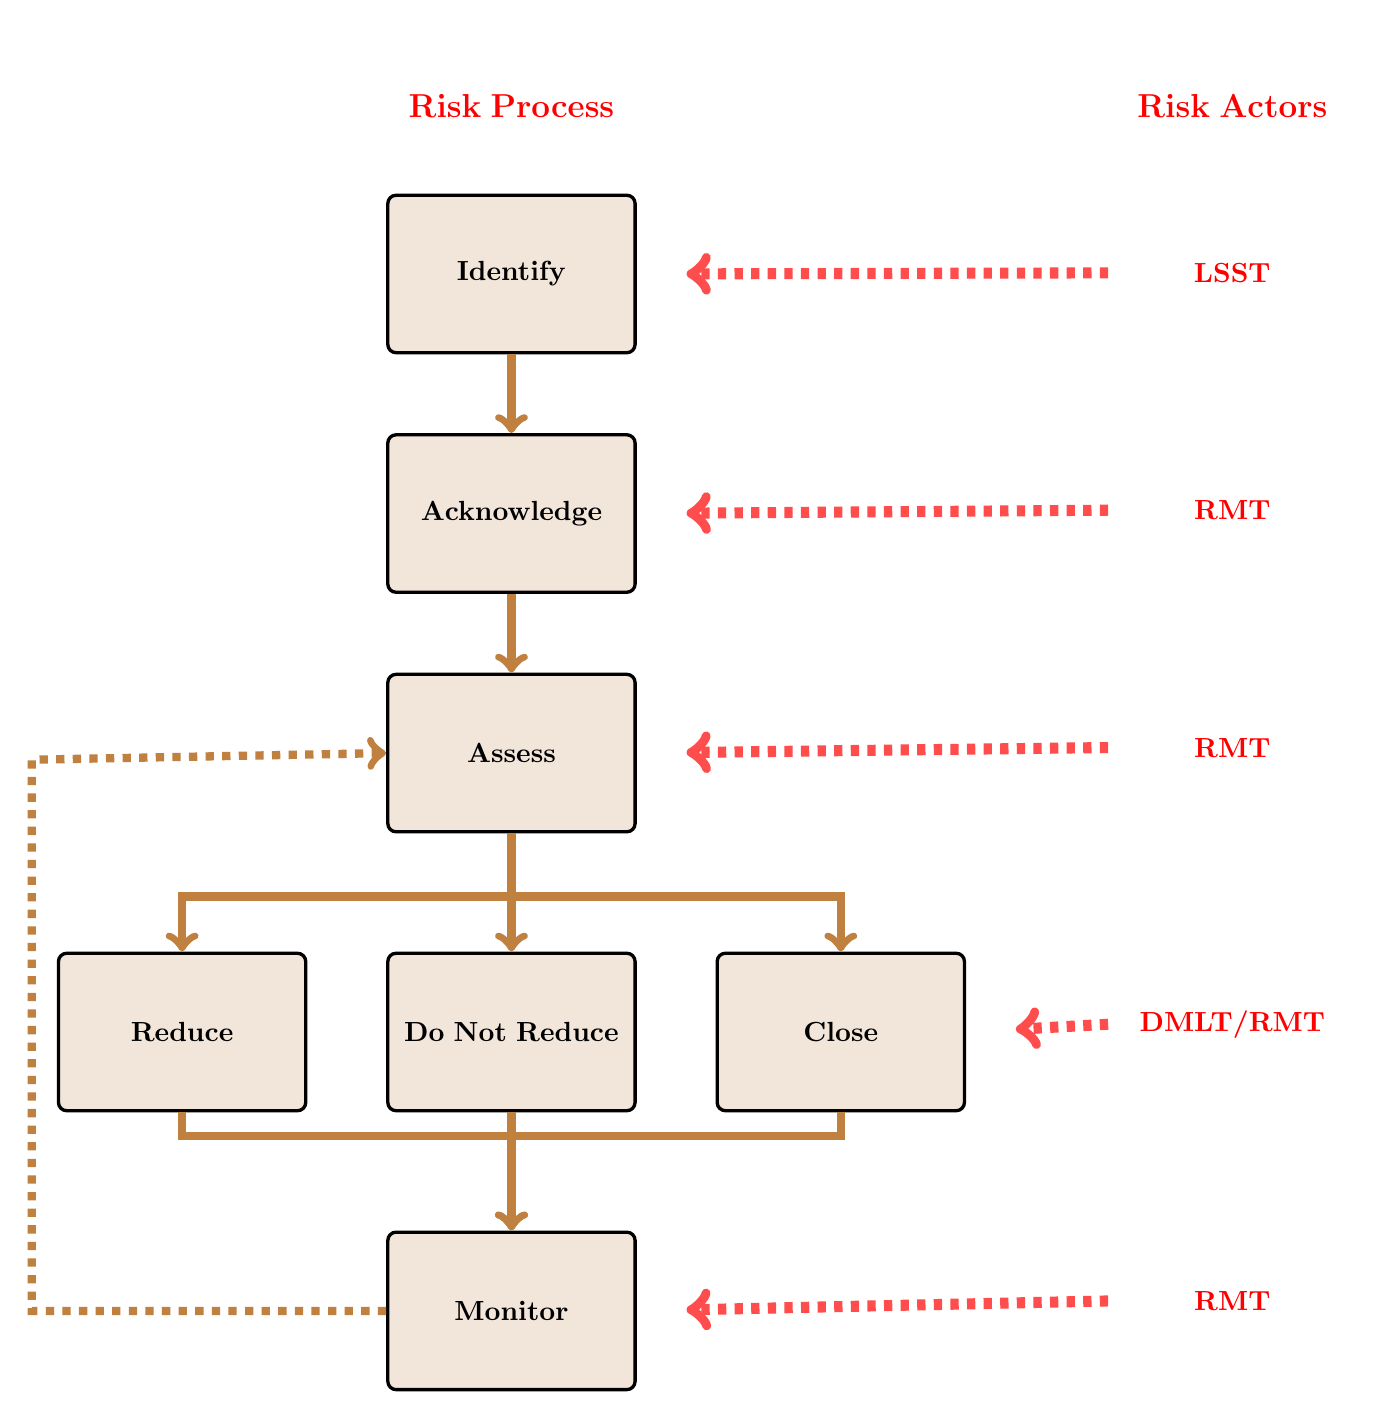
\begin{tikzpicture}[node distance=0mm]


    \node (rp) [abox, text width=3cm] 
	{ \large \textbf{Risk Process}
	};

    \node (id) [rbox, below=0.1cm of rp] {\textbf{Identify}};
    \node (ack) [rbox, below=1cm of id] {\textbf{Acknowledge}};
    \node (ass) [rbox, below=1cm of ack] {\textbf{Assess}};

    \node (act) [rectangle, below=0.8cm of ass,minimum width=12cm,minimum height=3.2cm, color=blue!50, dashed] {};

    \node (nred) [rbox, below=1.5cm of ass] {\textbf{Do Not Reduce}};
    \node (close) [rbox, right=1cm of nred] {\textbf{Close}};
    \node (red) [rbox, left=1cm of nred] {\textbf{Reduce}};

    \node (mon) [rbox, below=1.5cm of nred] {\textbf{Monitor}};

% Actors

    \node (ract) [abox, text width=3cm , right=6cm of rp] 
	{ \large \textbf{Risk Actors}
	};
    \node (lsst) [abox, text width=3cm , below=0.1cm of ract]  {\textbf{LSST}};
    \node (rmt) [abox, text width=3cm , below=1cm of lsst]  {\textbf{RMT}};
    \node (rmt2) [abox, text width=3cm , below=1cm of rmt]  {\textbf{RMT}};
    \node (dmlt) [abox, text width=3cm , below=1.5cm of rmt2]  {\textbf{DMLT/RMT}};
    \node (rmt3) [abox, text width=3cm , below=1.5cm of dmlt]  {\textbf{RMT}};

% lines
   \draw[pline] (id.south) -- (ack.north);
   \draw[pline] (ack.south) -- (ass.north);

   \draw[pline] (ass.south) -- (nred.north);
   \draw[pline] (ass.south) -- ++(0,-0.8) -| (red.north);
   \draw[pline] (ass.south) -- ++(0,-0.8) -| (close.north);

   \draw[pline] (red.south) -- ++(0,-0.3) -| (mon.north);
   \draw[pline] (close.south) -- ++(0,-0.3) -| (mon.north);

   \draw[pline] (nred.south) -- (mon.north);
   \draw[pdline] (mon.west) -- ++(-4.5,0) -- ++(0,7) --   (ass.west);
% actor lines
    
   \draw[rline] (lsst.west) -- (id.east) ;
   \draw[rline] (rmt.west) -- (ack.east) ;
   \draw[rline] (rmt2.west) -- (ass.east) ;
   \draw[rline] (dmlt.west) -- (close.east) ;
   \draw[rline] (rmt3.west) -- (mon.east) ;
\end{tikzpicture}
\end{document}
